%----------------------------------------------------------------------------------------
%	PACKAGES AND DOCUMENT CONFIGURATIONS
%----------------------------------------------------------------------------------------
\documentclass[article, a4paper, 12pt, oneside]{memoir}

% Margins
\usepackage[top=3cm,left=2cm,right=2cm,bottom=3cm]{geometry}

% Encondings
\usepackage[utf8]{inputenc}

% Language
\usepackage[portuguese]{babel}

% Graphics and images
\usepackage{graphicx}
	\graphicspath{{../images/}}

% Tables
\usepackage{tabularx}

% Paragraph Spacing
\usepackage{parskip}
\usepackage{indentfirst}
\setlength{\parskip}{0.5cm}

% Hyperreferences
\usepackage{hyperref}

% Repeated commands
\usepackage{expl3}
\ExplSyntaxOn
\cs_new_eq:NN \Repeat \prg_replicate:nn
\ExplSyntaxOff

% Header and Footer Things
\usepackage{wallpaper}
\usepackage{fancyhdr}

% Following code to edit the pagestyle
\pagestyle{fancy}
\fancyhf{}
\rhead{Hospital Database}
\lhead{\leftmark}
\rfoot{Página \thepage}

% Commands
\usepackage{xargs}

%% Linked Email
\newcommand{\email}[1]{
{\texttt{\href{mailto:#1}{#1}} }
}

%----------------------------------------------------------------------------------------
%	DOCUMENT INFORMATION
%----------------------------------------------------------------------------------------
% Title
\title{\Huge \texttt{Hospital Database (Parte 1)} }
% Authors
\author{
\LARGE \textbf{Grupo 406}\\\\
\begin{tabular}{l r}
	\email{up201806538@fe.up.pt} & Henrique Manuel Ruivo Pereira			\\
	\email{up201801011@fe.up.pt} & Iohan Xavier Sardinha Dutra Soares		\\
	\email{up201806554@fe.up.pt} & Telmo Alexandre Espirito Santo Baptista	\\
\end{tabular}
}

%\institute{Faculdade de Engenharia da Universidade do Porto \\ Bases de Dados (BDAD) - Turma 4, grupo 6}

% Date for the report
\date{\today}

% Table of Contents
\addto\captionsportuguese{\renewcommand*\contentsname{Índice}}

%----------------------------------------------------------------------------------------
%	DOCUMENT
%----------------------------------------------------------------------------------------
\begin{document}
%----------------------------------------------------------------------------------------
%	Front Page
%----------------------------------------------------------------------------------------
% Title Author and Date
\maketitle

% More information for front page
\begin{center}
\textbf{Projeto BDAD - 2019/20 - MIEIC}
\Repeat{2}{\linebreak}
\begin{tabular}{l r}
	\textbf{Professora das Aulas Laboratoriais}: & Carla Alexandra Teixeira Lopes
\end{tabular}
\Repeat{4}{\linebreak}
% FEUP Logo

\includegraphics[scale=0.4]{FEUP-logo.jpg}

\end{center}

\newpage
% Header Image
\CenterWallPaper{0.1}{FEUP-logo.jpg}
\addtolength{\wpXoffset}{-7.5cm}
\addtolength{\wpYoffset}{13.8cm}

%----------------------------------------------------------------------------------------
%	TABLE OF CONTENTS
%----------------------------------------------------------------------------------------
\tableofcontents*

\newpage
%----------------------------------------------------------------------------------------
%	CHAPTER 1 - Contexto
%----------------------------------------------------------------------------------------
\chapter[Contexto][Contexto]{Contexto} \label{\thechapter}
É pretendido modelar uma base de dados para um hospital com diversos tipos de serviços disponíveis.

O hospital é constituído por vários departamentos. Cada um destes tem nome, identificador, especializações e entidade responsável pelo departamento.

Staff e pacientes são pessoas, acerca das quais interessa saber o nome, o seu número de identificação único (cartão de cidadão ou equivalente), a sua morada, o seu contacto telefónico, o seu número de beneficiário, o seu sexo e a sua data de nascimento.

A entidade responsável por um departamento é um membro da staff do hospital, podendo este tratar-se de um médico, enfermeiro ou técnico no hospital. Cada membro do staff tem o seu código identificador no hospital.

Especificamente sobre os médicos, é necessário guardar o número do seu consultório no hospital (caso tenha) e a sua especialização (caso tenha).
Sobre os enfermeiros e os técnicos, apenas é necessário guardar a sua especialização (caso tenha).

O hospital guarda informação sobre os seus pacientes como o seu grupo sanguíneo, o subsistema de saúde ao qual o paciente está associado, o histórico das ocorrências de doenças que o paciente teve, os médicos atribuídos naquele hospital, e as suas admissões no hospital.

Sobre cada doença interessa guardar o seu nome, uma descrição da doença e os seus sintomas predominantes.

Uma admissão no hospital tem uma data, se se trata de uma admissão de urgência e, caso seja uma urgência, a prioridade desta. Uma admissão pode desencadear vários tipos de eventos. Cada evento tem uma descrição sobre do que se trata, uma data, o quarto onde se realiza e outras informações dependendo do tipo de evento, que pode corresponder a: uma consulta, um exame, uma intervenção ou um internamento.

Numa consulta, interessa guardar o médico que a realizou e o diagnóstico da consulta.
Num exame, guarda-se o nome do exame feito e uma descrição deste, bem como os médicos, enfermeiros e técnicos que dele participaram.
Numa intervenção, guarda-se uma descrição da intervenção realizada, bem como os médicos, enfermeiros e técnicos envolvidos.
Num internamento é necessário guardar o motivo deste, se ainda está ativo e, em caso negativo, a data na qual o paciente recebeu alta (saiu do internamento) caso tal já tenha acontecido.

\newpage
%----------------------------------------------------------------------------------------
%	CHAPTER 2 - UML
%----------------------------------------------------------------------------------------
\chapter[UML - Modelo Conceptual][UML]{UML - Modelo Conceptual} \label{\thechapter}
\hspace*{-1.3cm}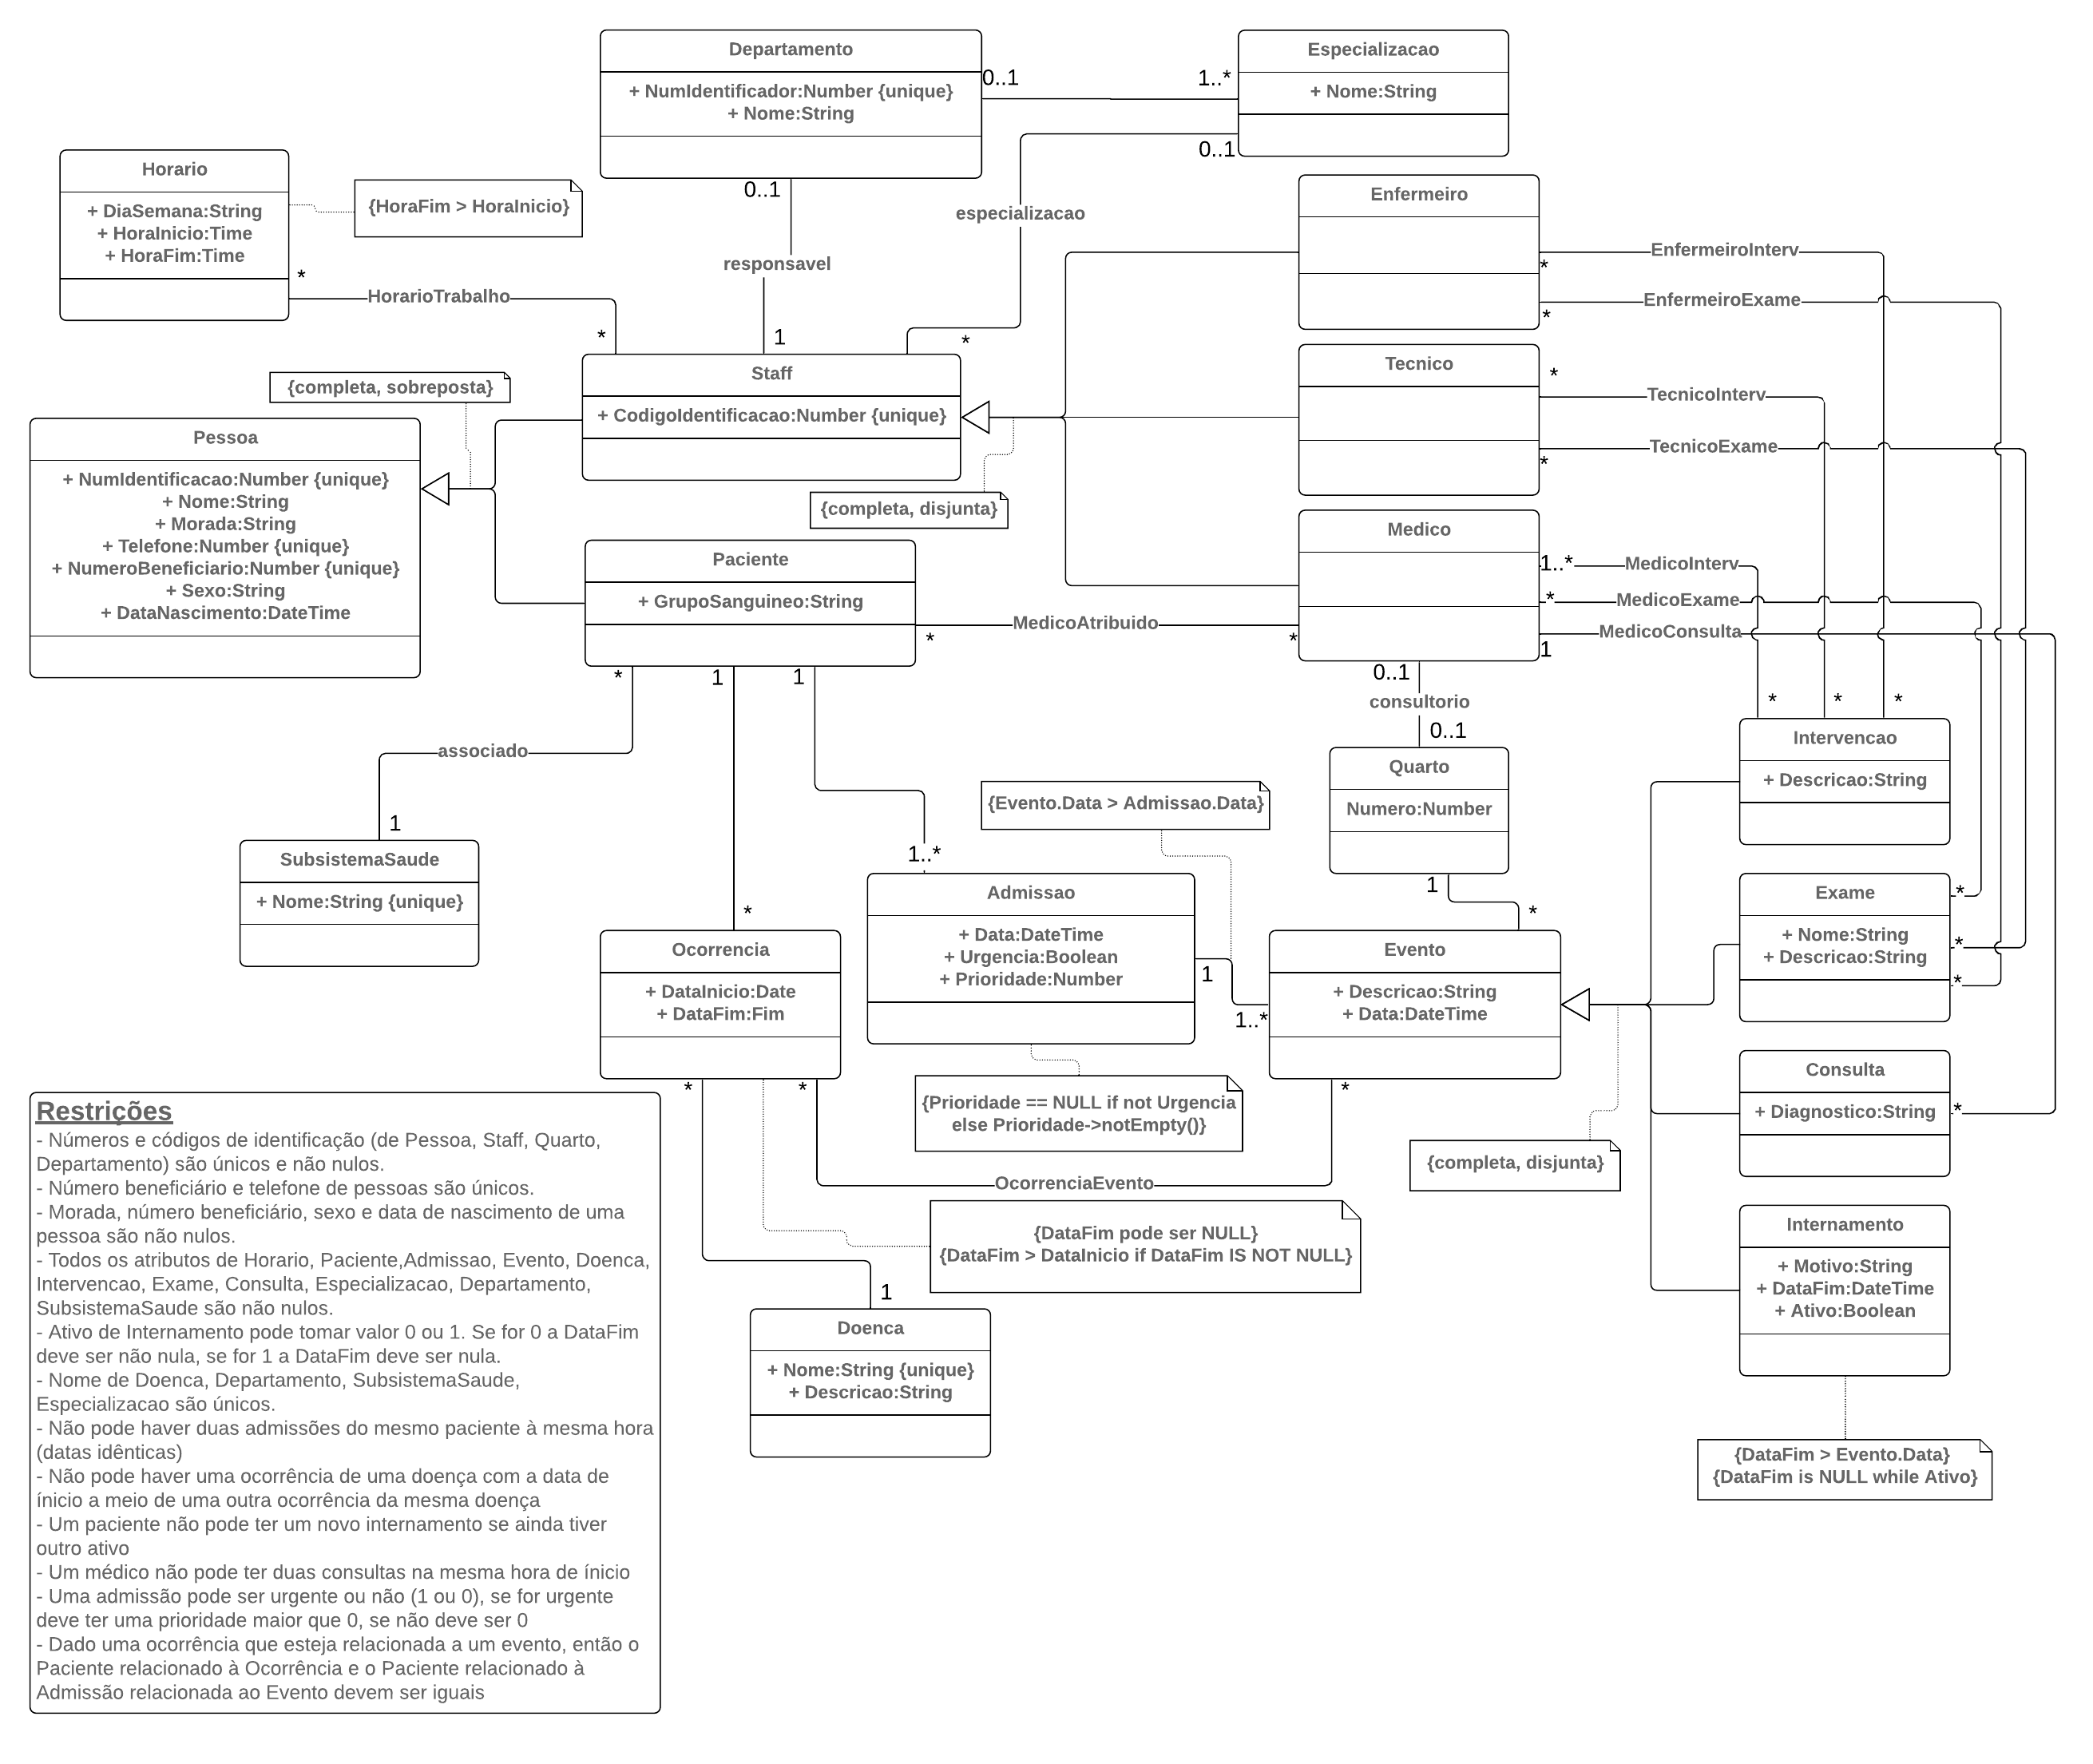
\includegraphics[width=1.1\linewidth, height=1.0\linewidth]{BDAD-UML.png}

\newpage
%----------------------------------------------------------------------------------------
%	CHAPTER 3 - Relational Model
%----------------------------------------------------------------------------------------
\chapter[Modelo Relacional][Modelo Relacional]{Modelo Relacional} \label{\thechapter}

\section{Classes}
\subsection{Classe Pessoa}
\begin{itemize}
	\item Pessoa(\underline{PessoaID}, NumIdentificacao, Nome, Morada, Telefone, NumeroBeneficiario, Sexo, DataNascimento)
\end{itemize}
\subsubsection{Classe Staff}
\begin{itemize}
	\item Staff(\underline{PessoaID}$\rightarrow$Pessoa, CodigoIdentificacao, Especializacao$\rightarrow$Especializacao)
	\begin{itemize}
		\item Enfermeiro(\underline{StaffID}$\rightarrow$Staff)
		\item Tecnico(\underline{StaffID}$\rightarrow$Staff)
		\item Medico(\underline{StaffID}$\rightarrow$Staff, Consultorio$\rightarrow$Quarto)
	\end{itemize}
	\item Especializacao(\underline{EspecializacaoID}, Nome, Departamento$\rightarrow$Departamento)
	\item Horario(\underline{HorarioID}, DiaSemana, HoraInicio, HoraFim)
	\item Departamento(\underline{NumIdentificador}, Nome, Responsavel$\rightarrow$Staff)
\end{itemize}
\subsubsection{Classe Paciente}
\begin{itemize}
	\item Paciente(\underline{PessoaID}$\rightarrow$Pessoa, GrupoSanguineo, SubsistemaSaude$\rightarrow$SubsistemaSaude)
	\item SubsistemaSaude(\underline{SubsistemaSaudeID}, Nome)
\end{itemize}
\subsection{Classe Evento}
\begin{itemize}
	\item Admissao(\underline{AdmissaoID}, Data, Urgencia, Prioridade, Paciente$\rightarrow$Paciente)
	\item Doenca(\underline{DoencaID}, Nome, Descricao, Sintomas)
	\item Ocorrencia(\underline{OcorrenciaID}, DataInicio, DataFim, Paciente$\rightarrow$Paciente, Doenca$\rightarrow$Doenca)
	\item Quarto(\underline{Numero})
	\item Evento(\underline{EventoID}, Descricao, Data, Admissao$\rightarrow$Admissao, Quarto$\rightarrow$Quarto)
	\begin{itemize}
		\item Intervencao(\underline{EventoID}$\rightarrow$Evento, Descricao)
		\item Exame(\underline{EventoID}$\rightarrow$Evento, Nome, Descricao)
		\item Consulta(\underline{EventoID}$\rightarrow$Evento, Diagnostico, Medico$\rightarrow$Medico)
		\item Internamento(\underline{EventoID}$\rightarrow$Evento, Motivo, DataFim, Ativo)
	\end{itemize}
\end{itemize}

\section{Associações}
\subsection{Associações muitos-para-muitos}
Associações relativas à classe Staff:
\begin{itemize}
	\item HorarioTrabalho(\underline{StaffID}$\rightarrow$Staff, \underline{HorarioID}$\rightarrow$Horario)
\end{itemize}

Associações relativas à classe Paciente:
\begin{itemize}
	\item MedicoAtribuido(\underline{PacienteID}$\rightarrow$Paciente, \underline{MedicoID}$\rightarrow$Medico)
\end{itemize}

Associações relativas à classe Evento:
\begin{itemize}
	\item EnfermeiroInterv(\underline{EnfermeiroID}$\rightarrow$Enfermeiro, \underline{IntervID}$\rightarrow$Intervencao)
	\item EnfermeiroExame(\underline{EnfermeiroID}$\rightarrow$Enfermeiro, \underline{ExameID}$\rightarrow$Exame)
	\item TecnicoInterv(\underline{TecnicoID}$\rightarrow$Tecnico, \underline{IntervID}$\rightarrow$Intervencao)
	\item TecnicoExame(\underline{TecnicoID}$\rightarrow$Tecnico, \underline{ExameID}$\rightarrow$Exame)
	\item MedicoInterv(\underline{MedicoID}$\rightarrow$Medico, \underline{IntervID}$\rightarrow$Intervencao)
	\item MedicoExame(\underline{MedicoID}$\rightarrow$Medico, \underline{ExameID}$\rightarrow$Exame)
	\item OcorrenciaEvento(\underline{OcorrenciaID}$\rightarrow$Ocorrencia, \underline{EventoID}$\rightarrow$Evento)
\end{itemize}

\subsection{Associações muitos-para-um}
Para este tipo de associações foi adotado o método de adicionar uma chave estrangeira para a relação do lado "um" na relação do lado "muitos".

\subsection{Associações um-para-um}
Para este tipo de associações foi adicionada uma chave estrangeira à relação que possuiria o menor número de tuplos, exceto nos casos em que essa relação pudesse ter esse elemento como nulo, nos casos em que ambos podem ser nulos.

\section{Generalizações}
Quanto às generalizações, optou-se por usar o método E/R, criando uma relação para cada classe, e adicionando a chave da super-classe às subclasses, devido às restrições que necessitam ser implementadas nestas classes.

\newpage
%----------------------------------------------------------------------------------------
%	CHAPTER 4 - Analysis of Functional Dependencies and Normal Forms
%----------------------------------------------------------------------------------------
\chapter[Análise de DFs e FNs][Análise de DFs e FNs]{Análise de Dependências Funcionais e Formas Normais} \label{\thechapter}

Para cada relação será estudado se esta se encontra na forma normal Boyce-Codd e na 3ª forma normal.

\textbf{Forma normal Boyce-Codd (BCNF)}\\
Uma relação $R$ com dependências funcionais $FD$ está na forma normal de Boyce-Codd se:
\begin{itemize}
	\item Para cada dependência funcional não trivial $\overline{A}\rightarrow\overline{B}$, $\overline{A}$ é uma (super)chave da relação R.
\end{itemize}

\textbf{Terceira forma normal (3NF)}\\
Uma relação $R$ com dependências funcionais $FD$ está na terceira forma normal se:
\begin{itemize}
	\item Para cada dependência funcional não trivial $\overline{A}\rightarrow\overline{B}$, se se verificar pelo menos uma das seguintes propriedades:
	\begin{itemize}
		\item $\overline{A}$ é uma (super)chave da relação R;
		\item $\overline{B}$ consiste apenas de atributos primos (atributos que pertencem a pelo menos uma chave).
	\end{itemize}
\end{itemize}

Vale notar que se uma relação estiver na forma normal Boyce-Codd (BCNF), esta também se encontra na terceira forma normal (3NF), já que as 3NF são um superconjunto das BCNF\\
Se uma relação apenas consistir de dependências funcionais triviais, então a relação também está na forma normal de Boyce-Codd e por consequência na terceira forma normal.

\newpage

\section*{Pessoa}
\begin{itemize}
	\item PessoaID$\rightarrow$NumIdentificacao, Nome, Morada, Telefone, NumeroBeneficiario, Sexo, DataNascimento
	\item NumIdentificacao$\rightarrow$PessoaID, Nome, Morada, Telefone, NumeroBeneficiario, Sexo, DataNascimento
	\item Telefone$\rightarrow$PessoaID, NumIdentificacao, Nome, Morada, NumeroBeneficiario, Sexo, DataNascimento
	\item NumeroBeneficiario$\rightarrow$PessoaID, NumIdentificacao, Nome, Morada, Telefone, Sexo, DataNascimento
\end{itemize}

\textbf{Chaves candidatas}:\\
\[
\{ PessoaID \}, \{ NumIdentificacao \}, \{ Telefone \}, \{ NumeroBeneficiario \}
\]
Como, para cada dependência não trivial, o conjunto de atributos no lado esquerdo (\underline{A}) é composto por uma key, então esta relação está na forma normal de Boyce-Codd (BCNF) e por consequência também se encontra na terceira forma normal (3NF)

\section*{Staff}
\begin{itemize}
	\item PessoaID$\rightarrow$CodigoIdentificacao, Especializacao
	\item CodigoIdentificacao$\rightarrow$PessoaID, Especializacao
\end{itemize}

\textbf{Chaves candidatas}:\\
\[
\{ PessoaID \}, \{ CodigoIdentificacao \}
\]

Como para cada dependência não trivial o conjunto de atributos no lado esquerdo (\underline{A}) é composto por uma key, então esta relação está na forma normal de Boyce-Codd (BCNF) e por consequência também se encontra na terceira form normal (3NF)

\section*{Enfermeiro}
Não tem dependências funcionais não triviais, logo, esta relação encontra-se na forma normal de Boyce-Codd (BCNF) e na terceira forma normal (3NF)

\section*{Tecnico}
Não tem dependências funcionais não triviais, logo, esta relação encontra-se na forma normal de Boyce-Codd (BCNF) e na terceira forma normal (3NF)

\section*{Medico}
\begin{itemize}
	\item StaffID$\rightarrow$Consultorio
	\item Consultorio$\rightarrow$StaffID
\end{itemize}

\textbf{Chaves candidatas}:\\
\[
\{ StaffID \}, \{ Consultorio \}
\]

Como para cada dependência não trivial o conjunto de atributos no lado esquerdo (\underline{A}) é composto por uma key, então esta relação está na forma normal de Boyce-Codd (BCNF) e por consequência também se encontra na terceira form normal (3NF)

\section*{Especializacao}
\begin{itemize}
	\item EspecializacaoID$\rightarrow$Nome, Departamento
	\item Nome$\rightarrow$EspecializacaoID, Departamento
\end{itemize}

\textbf{Chaves candidatas}:\\
\[
\{ EspecializacaoID \}, \{ Nome \}
\]

Como para cada dependência não trivial o conjunto de atributos no lado esquerdo (\underline{A}) é composto por uma key, então esta relação está na forma normal de Boyce-Codd (BCNF) e por consequência também se encontra na terceira form normal (3NF)

\newpage

\section*{Horario}
\begin{itemize}
	\item HorarioID$\rightarrow$DiaSemana, HoraInicio, HoraFim
\end{itemize}

\textbf{Chaves candidatas}:\\
\[
\{ HorarioID \}
\]

Como para cada dependência não trivial o conjunto de atributos no lado esquerdo (\underline{A}) é composto por uma key, então esta relação está na forma normal de Boyce-Codd (BCNF) e por consequência também se encontra na terceira form normal (3NF)

\section*{Departamento}
\begin{itemize}
	\item NumIdentificador$\rightarrow$Nome, Responsavel
	\item Responsavel$\rightarrow$NumIdentificador, Nome
\end{itemize}

\textbf{Chaves candidatas}:\\
\[
\{ NumIdentificador \}, \{ Responsavel \}
\]

Como para cada dependência não trivial o conjunto de atributos no lado esquerdo (\underline{A}) é composto por uma key, então esta relação está na forma normal de Boyce-Codd (BCNF) e por consequência também se encontra na terceira form normal (3NF)

\section*{Paciente}
\begin{itemize}
	\item PessoaID$\rightarrow$GrupoSanguineo, SubsistemaSaude
\end{itemize}

\textbf{Chaves candidatas}:\\
\[
\{ PessoaID \}
\]

Como para cada dependência não trivial o conjunto de atributos no lado esquerdo (\underline{A}) é composto por uma key, então esta relação está na forma normal de Boyce-Codd (BCNF) e por consequência também se encontra na terceira form normal (3NF)

\section*{SubsistemaSaude}
\begin{itemize}
	\item SubsistemaSaudeID$\rightarrow$Nome
	\item Nome$\rightarrow$SubsistemaSaudeID
\end{itemize}

\textbf{Chaves candidatas}:\\
\[
\{ SubsistemaSaudeID \}, \{ Nome \}
\]

Como para cada dependência não trivial o conjunto de atributos no lado esquerdo (\underline{A}) é composto por uma key, então esta relação está na forma normal de Boyce-Codd (BCNF) e por consequência também se encontra na terceira form normal (3NF)

\section*{Admissao}
\begin{itemize}
	\item AdmissaoID$\rightarrow$Data, Urgencia, Prioridade, Paciente
	\item Data, Paciente$\rightarrow$AdmissaoID, Urgencia, Prioridade
\end{itemize}

\textbf{Chaves candidatas}:\\
\[
\{ AdmissaoID \}, \{ Data, Paciente \}
\]

Como para cada dependência não trivial o conjunto de atributos no lado esquerdo (\underline{A}) é composto por uma key, então esta relação está na forma normal de Boyce-Codd (BCNF) e por consequência também se encontra na terceira form normal (3NF)

\section*{Doenca}
\begin{itemize}
	\item DoencaID$\rightarrow$Nome, Descricao, Sintomas
	\item Nome$\rightarrow$DoencaID, Descricao, Sintomas
\end{itemize}

\textbf{Chaves candidatas}:\\
\[
\{ DoencaID \}, \{ Nome \}
\]

Como para cada dependência não trivial o conjunto de atributos no lado esquerdo (\underline{A}) é composto por uma key, então esta relação está na forma normal de Boyce-Codd (BCNF) e por consequência também se encontra na terceira form normal (3NF)

\section*{Ocorrencia}
\begin{itemize}
	\item OcorrenciaID$\rightarrow$DataInicio, DataFim, Paciente, Doenca
	\item DataInicio, Paciente, Doenca$\rightarrow$OcorrenciaID, DataFim
\end{itemize}

\textbf{Chaves candidatas}:\\
\[
\{ OcorrenciaID \}, \{ DataInicio, Paciente, Doenca \}
\]

Como para cada dependência não trivial o conjunto de atributos no lado esquerdo (\underline{A}) é composto por uma key, então esta relação está na forma normal de Boyce-Codd (BCNF) e por consequência também se encontra na terceira form normal (3NF)

\section*{Quarto}
Não tem dependências funcionais.

\section*{Evento}
\begin{itemize}
	\item EventoID$\rightarrow$Descricao, Data, Admissao, Quarto
\end{itemize}

\textbf{Chaves candidatas}:\\
\[
\{ EventoID \}
\]

Como para cada dependência não trivial o conjunto de atributos no lado esquerdo (\underline{A}) é composto por uma key, então esta relação está na forma normal de Boyce-Codd (BCNF) e por consequência também se encontra na terceira form normal (3NF)

\newpage

\section*{Intervencao}
\begin{itemize}
	\item EventoID$\rightarrow$Descricao
\end{itemize}

\textbf{Chaves candidatas}:\\
\[
\{ EventoID \}
\]

Como para cada dependência não trivial o conjunto de atributos no lado esquerdo (\underline{A}) é composto por uma key, então esta relação está na forma normal de Boyce-Codd (BCNF) e por consequência também se encontra na terceira form normal (3NF)

\section*{Exame}
\begin{itemize}
	\item EventoID$\rightarrow$Nome, Descricao
\end{itemize}

\textbf{Chaves candidatas}:\\
\[
\{ EventoID \}
\]

Como para cada dependência não trivial o conjunto de atributos no lado esquerdo (\underline{A}) é composto por uma key, então esta relação está na forma normal de Boyce-Codd (BCNF) e por consequência também se encontra na terceira form normal (3NF)

\section*{Consulta}
\begin{itemize}
	\item EventoID$\rightarrow$Diagnostico, Medico
\end{itemize}

\textbf{Chaves candidatas}:\\
\[
\{ EventoID \}
\]

Como para cada dependência não trivial o conjunto de atributos no lado esquerdo (\underline{A}) é composto por uma key, então esta relação está na forma normal de Boyce-Codd (BCNF) e por consequência também se encontra na terceira form normal (3NF)

\section*{Internamento}
\begin{itemize}
	\item EventoID$\rightarrow$Motivo, DataFim, Ativo
\end{itemize}

\textbf{Chaves candidatas}:\\
\[
\{ EventoID \}
\]

Como para cada dependência não trivial o conjunto de atributos no lado esquerdo (\underline{A}) é composto por uma key, então esta relação está na forma normal de Boyce-Codd (BCNF) e por consequência também se encontra na terceira form normal (3NF)

\section*{HorarioTrabalho}
Não tem dependências funcionais não triviais, logo, esta relação encontra-se na forma normal de Boyce-Codd (BCNF) e na terceira forma normal (3NF)

\section*{MedicoAtribuido}
Não tem dependências funcionais não triviais, logo, esta relação encontra-se na forma normal de Boyce-Codd (BCNF) e na terceira forma normal (3NF)

\section*{EnfermeiroInterv}
Não tem dependências funcionais não triviais, logo, esta relação encontra-se na forma normal de Boyce-Codd (BCNF) e na terceira forma normal (3NF)

\section*{EnfermeiroExame}
Não tem dependências funcionais não triviais, logo, esta relação encontra-se na forma normal de Boyce-Codd (BCNF) e na terceira forma normal (3NF)

\section*{TecnicoInterv}
Não tem dependências funcionais não triviais, logo, esta relação encontra-se na forma normal de Boyce-Codd (BCNF) e na terceira forma normal (3NF)

\section*{TecnicoExame}
Não tem dependências funcionais não triviais, logo, esta relação encontra-se na forma normal de Boyce-Codd (BCNF) e na terceira forma normal (3NF)

\section*{MedicoInterv}
Não tem dependências funcionais não triviais, logo, esta relação encontra-se na forma normal de Boyce-Codd (BCNF) e na terceira forma normal (3NF)

\section*{MedicoExame}
Não tem dependências funcionais não triviais, logo, esta relação encontra-se na forma normal de Boyce-Codd (BCNF) e na terceira forma normal (3NF)

\section*{OcorrenciaEvento}
Não tem dependências funcionais não triviais, logo, esta relação encontra-se na forma normal de Boyce-Codd (BCNF) e na terceira forma normal (3NF)

\newpage
%----------------------------------------------------------------------------------------
%	CHAPTER 5 - Restrictions
%----------------------------------------------------------------------------------------
\chapter[Restrições][Restrições]{Restrições} \label{\thechapter}

\section*{Pessoa}
\begin{itemize}
	\item cada pessoa tem um ID único (\textbf{PRIMARY KEY})
	\item cada pessoa deve ter um número de identificação, nome, morada, número de beneficiário, telefone, sexo e data de nascimento (\textbf{NOT NULL})
	\item o número de identificação e o número de beneficiário devem ser únicos (\textbf{UNIQUE})
\end{itemize}

\section*{Staff}
\begin{itemize}
	\item cada membro da staff tem um ID único (\textbf{PRIMARY KEY})
	\item além disso, PessoaID é chave estrangeira para Pessoa (\textbf{FOREIGN KEY})
	\item não é possível eliminar uma pessoa enquanto houver staff mapeada para essa pessoa, mas pode-se alterar a pessoa que alterará na staff que a mapeia (\textbf{ON DELETE RESTRICT} e \textbf{ON UPDATE CASCADE})
	\item Especializacao é chave estrangeira para Especializacao, e tal será posta a \textbf{NULL} caso a Especializacao seja eliminada, em caso de alterações, as alterações seram feitas em toda a staff que mapeia essa especialização (\textbf{ON DELETE SET NULL} e \textbf{ON UPDATE CASCADE})
\end{itemize}

\subsubsection*{Enfermeiro}
\begin{itemize}
	\item cada enfermeiro tem o seu ID (\textbf{StaffID}) que é chave estrangeira para Staff (\textbf{FOREIGN KEY})
	\item além disso, este ID deve ser único (\textbf{PRIMARY KEY})
	\item não é possível eliminar um membro da staff enquanto houver um enfermeiro mapeado para esse membro da staff, mas pode-se alterar a staff que alterará também no enfermeiro que a mapeia (\textbf{ON DELETE RESTRICT} e \textbf{ON UPDATE CASCADE})
\end{itemize}

\newpage

\subsubsection*{Tecnico}
\begin{itemize}
	\item cada técnico tem o seu ID (\textbf{StaffID}) que é chave estrangeira para Staff (\textbf{FOREIGN KEY})
	\item além disso, este ID deve ser único (\textbf{PRIMARY KEY})
	\item não é possível eliminar um membro da staff enquanto houver um técnico mapeado para esse membro da staff, mas pode-se alterar a staff que alterará também no técnico que a mapeia (\textbf{ON DELETE RESTRICT} e \textbf{ON UPDATE CASCADE})
\end{itemize}

\subsubsection*{Medico}
\begin{itemize}
	\item cada médico tem o seu ID (\textbf{StaffID}) que é chave estrangeira para Staff (\textbf{FOREIGN KEY})
	\item além disso, este ID deve ser único (\textbf{PRIMARY KEY})
	\item não é possível eliminar um membro da staff enquanto houver um médico mapeado para esse membro da staff, mas pode-se alterar a staff que alterará também no médico que a mapeia (\textbf{ON DELETE RESTRICT} e \textbf{ON UPDATE CASCADE})
	\item Consultorio é chave estrangeira para Quarto (\textbf{FOREIGN KEY})
	\item o consultório deve ser único (\textbf{UNIQUE})
	\item caso se elimine um quarto que é mapeado como consultório, o valor do consultório é colocado a nulo, em caso de alteração, o consultório também é alterado (\textbf{ON DELETE SET NULL} e \textbf{ON UPDATE CASCADE})
\end{itemize}

\section*{Especializacao}
\begin{itemize}
	\item cada especialização deve ter um ID único (\textbf{PRIMARY KEY})
	\item nome da especialização deve ser único e não nulo (\textbf{NOT NULL} e \textbf{UNIQUE})
	\item Departamento é chave estrangeira para Departamento
	\item caso se elimine um departamento, será colocado a nulo o valor do departamento em todas as especializações que o mapeiem, em caso de alteração, será alterado também (\textbf{ON UPDATE CASCADE} e \textbf{ON DELETE SET NULL})
\end{itemize}

\newpage

\section*{Horario}
\begin{itemize}
	\item cada horário tem um ID único (\textbf{PRIMARY KEY})
	\item cada horário deve ter um dia da semana correspondente, uma hora de início e uma hora de fim (\textbf{NOT NULL})
	\item a hora de início deve ser antes da hora de fim (\textbf{CHECK})
\end{itemize}

\section*{Departamento}
\begin{itemize}
	\item cada departamento tem o seu número identificador único (\textbf{PRIMARY KEY})
	\item cada departamento tem um nome e um responsável (\textbf{NOT NULL})
	\item Responsavel é chave estrangeira para staff (\textbf{FOREIGN KEY})
	\item não é possível remover um membro da staff caso esse esteja mapeado como um Responsavel de um departamento, mas é possível alterá-lo, tais alterações serão aplicadas no departamento que mapeia o membro da staff (\textbf{ON DELETE RESTRICT} e \textbf{ON UPDATE CASCADE})
	\item não pode haver dois departamentos com um mesmo membro da staff responsável (\textbf{UNIQUE})
\end{itemize}

\section*{Paciente}
\begin{itemize}
	\item cada paciente tem um número de identificação único (\textbf{PRIMARY KEY})
	\item além disso, número de identificação (\textbf{PessoaID}) é chave estrangeira para Pessoa (\textbf{FOREIGN KEY})
	\item não é possível eliminar uma pessoa enquanto houver um paciente mapeada para essa pessoa, mas pode-se alterar a pessoa que alterará no paciente que a mapeia (\textbf{ON DELETE RESTRICT} e \textbf{ON UPDATE CASCADE})
	\item cada paciente tem um grupo sanguineo (\textbf{NOT NULL})
	\item SubsistemaSaude é chave estrangeira para SubsistemaSaude (\textbf{FOREIGN KEY})
	\item ao eliminar um subsistema de saúde colocará em todos os pacientes que o mapeavam o valor \textbf{NULL}, em caso de alteração, alterará também no paciente que o mapeia (\textbf{ON DELETE SET NULL} e \textbf{ON UPDATE CASCADE})
\end{itemize}

\section*{SubsistemaSaude}
\begin{itemize}
	\item cada subsistema de saúde tem um ID único (\textbf{PRIMARY KEY})
	\item nome do subsistema de saúde deve ser único e não nulo (\textbf{NOT NULL} e \textbf{UNIQUE})
\end{itemize}

\section*{Admissao}
\begin{itemize}
	\item cada admissão tem um ID único (\textbf{PRIMARY KEY})
	\item cada admissão tem uma data e um paciente (\textbf{NOT NULL})
	\item uma admissão pode ser urgência ou não (isto é, tem o valor 1 ou 0, respetivamente), por omissão trata-se de uma admissão não urgente (\textbf{NOT NULL}, \textbf{CHECK} e \textbf{DEFAULT})
	\item caso seja uma admissão de urgência a prioridade deve ter um valor maior que 0, em caso não urgente, a prioridade por omissão é 0 (\textbf{NOT NULL}, \textbf{CHECK} e \textbf{DEFAULT})
	\item Paciente é chave estrangeira para Paciente (\textbf{FOREIGN KEY})
	\item não é possível eliminar um paciente caso este esteja mapeado em Admissao, e alterar um paciente altera também em Admissao (\textbf{ON UPDATE CASCADE} e \textbf{ON DELETE RESTRICT})
	\item um paciente não pode ter duas admissões na mesma hora do mesmo dia (datas idênticas) (\textbf{UNIQUE})
\end{itemize}

\section*{Doenca}
\begin{itemize}
	\item cada doença tem um ID único (\textbf{PRIMARY KEY})
	\item cada doença tem um nome, uma descrição e os seus sintomas (\textbf{NOT NULL})
	\item o nome da doença deve ser único (\textbf{UNIQUE})
\end{itemize}

\newpage

\section*{Ocorrencia}
\begin{itemize}
	\item cada ocorrência tem um ID único (\textbf{PRIMARY KEY})
	\item cada ocorrência tem uma data ínicio, um paciente e uma doença associada à ocorrência (\textbf{NOT NULL})
	\item Paciente é chave estrangeira para Paciente, Doenca é chave estrangeira para Doenca (\textbf{REFERENCES})
	\item não é possível eliminar uma doença ou um paciente se houver ocorrências a mapeá-los, mas ao alterar os mesmos, a informação também será alterada nas ocorrências que os mapeiam (\textbf{ON DELETE RESTRICT} e \textbf{ON UPDATE CASCADE})
	\item se a data de fim for não nula, então deve ser depois da data de ínicio (\textbf{CHECK})
	\item não pode haver ínicio de uma ocorrência de uma doença a meio de uma ocorrência dessa mesma doença (\textbf{TRIGGER}) (esta restrição foi implementada, nesta entrega, apenas considerando datas de ínicio iguais)
\end{itemize}

\section*{Quarto}
\begin{itemize}
	\item cada quarto tem um número único (\textbf{PRIMARY KEY})
\end{itemize}

\section*{Evento}
\begin{itemize}
	\item cada evento tem um ID único (\textbf{PRIMARY KEY})
	\item cada admissão tem uma descrição e uma data, a admissão ao qual está relacionada e o quarto onde foi procedido esse evento (\textbf{NOT NULL})
	\item Admissao é chave estrangeira para Admissao, Quarto é chave estrangeira para Quarto (\textbf{FOREIGN KEY})
	\item não é possível eliminar uma admissão nem um quarto enquanto houver ocorrências a mapeá-los, em caso de alteração, estas também são aplicadas nas ocorrências que os mapeiam (\textbf{ON DELETE RESTRICT} e \textbf{ON UPDATE CASCADE})
	\item a data do evento deve ser maior que a data de admissão (\textbf{TRIGGER})
\end{itemize}

\newpage

\section*{Invervencao}
\begin{itemize}
	\item cada intervenção tem um ID (do evento) único (\textbf{PRIMARY KEY})
	\item cada intervenção tem uma descrição (\textbf{NOT NULL})
	\item o ID da intervenção (\textbf{EventoID}) é chave estrangeira para Evento (\textbf{FOREIGN KEY})
	\item não é possível eliminar um evento se houver uma intervenção que o mapeia, em caso de alterações, estas também são aplicadas nas intervenções que os mapeiam (\textbf{ON DELETE RESTRICT} e \textbf{ON UPDATE CASCADE})
\end{itemize}

\section*{Exame}
\begin{itemize}
	\item cada exame deve ter um ID (do evento) único (\textbf{PRIMARY KEY})
	\item cada exame tem um nome e uma descrição (\textbf{NOT NULL})
	\item o ID do exame (\textbf{EventoID}) é chave estrangeira para Evento (\textbf{FOREIGN KEY})
	\item não é possível eliminar um evento se houver um exame que o mapeia, em caso de alterações, estas também são aplicadas nos exames que os mapeiam (\textbf{ON DELETE RESTRICT} e \textbf{ON UPDATE CASCADE})
\end{itemize}

\section*{Consulta}
\begin{itemize}
	\item cada consulta deve ter um ID (do evento) único (\textbf{PRIMARY KEY})
	\item cada consulta tem um médico associado e um diagnóstico (\textbf{NOT NULL})
	\item o ID da consulta (\textbf{EventoID}) é chave estrangeira para Evento, Medico é chave estrangeira para Medico (\textbf{FOREIGN KEY})
	\item não é possível eliminar um evento se houver uma consulta que o mapeia, em caso de alterações, estas também são aplicadas nas consulta que os mapeiam. O mesmo se aplica para a chave estrangeira Medico (\textbf{ON DELETE RESTRICT} e \textbf{ON UPDATE CASCADE})
	\item um médico não pode ter duas consultas na mesma hora de ínicio (\textbf{TRIGGER})
\end{itemize}

\newpage

\section*{Internamento}
\begin{itemize}
	\item cada internamento deve ter um ID (do evento) único (\textbf{PRIMARY KEY})
	\item cada internamento tem um motivo e se o internamento está ativo ou não (\textbf{NOT NULL})
	\item o ID do internamento (\textbf{EventoID}) é chave estrangeira para Evento (\textbf{FOREIGN KEY})
	\item não é possível eliminar um evento se houver um internamento que o mapeia, em caso de alterações, estas também são aplicadas nos internamento que os mapeiam (\textbf{ON DELETE RESTRICT} e \textbf{ON UPDATE CASCADE})
	\item Ativo é um valor booleano, tomando o valor de 0 ou 1 (\textbf{CHECK})
	\item se Ativo estiver a 1 então DataFim deve ser não nula, se tiver a 0 então DataFim deve ser nula (\textbf{CHECK})
	\item DataFim deve ser maior que a Data do evento mapeado na chave estrangeira EventoID (\textbf{TRIGGER})
	\item um paciente não pode ter um novo internamento se tiver um ativo (\textbf{TRIGGER})
\end{itemize}

\section*{HorarioTrabalho}
\begin{itemize}
	\item cada intermante deve ter um ID de staff e um ID de horário único (\textbf{PRIMARY KEY})
	\item StaffID é chave estrangeira para Staff e HorarioID chave estrangeira para Horario (\textbf{REFERENCES})
	\item ao eliminar uma staff que esteja mapeada num HorarioTrabalho, eliminará também o HorarioTrabalho, em caso de alteração, também alterará em HorarioTrabalho. O mesmo aplica-se à chave estrangeira Horario (\textbf{ON DELETE CASCADE} e \textbf{ON UPDATE CASCADE})
\end{itemize}

\section*{MedicoAtribuido}
\begin{itemize}
	\item cada intermante deve ter um ID de um paciente e um ID de um médico único (\textbf{PRIMARY KEY})
	\item PacienteID é chave estrangeira para Paciente e MedicoID chave estrangeira para Medico (\textbf{FOREIGN KEY})
	\item ao eliminar um paciente que esteja mapeada num MedicoAtribuido, eliminará também o MedicoAtribuido, em caso de alteração, também alterará em MedicoAtribuido. O mesmo aplica-se à chave estrangeira MedicoID (\textbf{ON DELETE CASCADE} e \textbf{ON UPDATE CASCADE})
\end{itemize}

\section*{EnfermeiroInterv}
\begin{itemize}
	\item deve ter uma intervenção ao qual foi atribuído um enfermeiro (\textbf{PRIMARY KEY})
	\item EnfermeiroID é uma chave estrangeira para Enfermeiro e IntervID é chave estrangeira para Intervencao
	\item ao eliminar um enfermeiro que esteja mapeado num EnfermeiroInterv, eliminará também o EnfermeiroInterv, em caso de alteração, também alterará em EnfermeiroInterv. O mesmo aplica-se à chave estrangeira IntervID (\textbf{ON DELETE CASCADE} e \textbf{ON UPDATE CASCADE})
\end{itemize}

\section*{EnfermeiroExame}
\begin{itemize}
	\item deve ter um exame ao qual foi atribuído um enfermeiro (\textbf{PRIMARY KEY})
	\item EnfermeiroID é uma chave estrangeira para Enfermeiro e ExameID é chave estrangeira para Exame
	\item ao eliminar um enfermeiro que esteja mapeado num EnfermeiroExame, eliminará também o EnfermeiroExame, em caso de alteração, também alterará em EnfermeiroExame. O mesmo aplica-se à chave estrangeira ExameID (\textbf{ON DELETE CASCADE} e \textbf{ON UPDATE CASCADE})
\end{itemize}

\section*{TecnicoInterv}
\begin{itemize}
	\item deve ter uma intervenção ao qual foi atribuído um técnico (\textbf{PRIMARY KEY})
	\item TecnicoID é uma chave estrangeira para Tecnico e IntervID é chave estrangeira para Intervencao
	\item ao eliminar um técnico que esteja mapeado num TecnicoInterv, eliminará também o TecnicoInterv, em caso de alteração, também alterará em TecnicoInterv. O mesmo aplica-se à chave estrangeira IntervID (\textbf{ON DELETE CASCADE} e \textbf{ON UPDATE CASCADE})
\end{itemize}

\newpage

\section*{TecnicoExame}
\begin{itemize}
	\item deve ter um exame ao qual foi atribuído um técnico (\textbf{PRIMARY KEY})
	\item TecnicoID é uma chave estrangeira para Tecnico e ExameID é chave estrangeira para Exame
	\item ao eliminar um técnico que esteja mapeado num TecnicoExame, eliminará também o TecnicoExame, em caso de alteração, também alterará em TecnicoExame. O mesmo aplica-se à chave estrangeira ExameID (\textbf{ON DELETE CASCADE} e \textbf{ON UPDATE CASCADE})
\end{itemize}

\section*{MedicoInterv}
\begin{itemize}
	\item deve ter uma intervenção ao qual foi atribuído um médico (\textbf{PRIMARY KEY})
	\item MedicoID é uma chave estrangeira para Medico e IntervID é chave estrangeira para Intervencao
	\item ao eliminar um médico que esteja mapeado num MedicoInterv, eliminará também o MedicoInterv, em caso de alteração, também alterará em MedicoInterv. O mesmo aplica-se à chave estrangeira IntervID (\textbf{ON DELETE CASCADE} e \textbf{ON UPDATE CASCADE})
\end{itemize}

\section*{MedicoExame}
\begin{itemize}
	\item deve ter um exame ao qual foi atribuído um médico (\textbf{PRIMARY KEY})
	\item MedicoID é uma chave estrangeira para Medico e ExameID é chave estrangeira para Exame
	\item ao eliminar um médico que esteja mapeado num MedicoExame, eliminará também o MedicoExame, em caso de alteração, também alterará em MedicoExame. O mesmo aplica-se à chave estrangeira ExameID (\textbf{ON DELETE CASCADE} e \textbf{ON UPDATE CASCADE})
\end{itemize}

\newpage

\section*{OcorrenciaEvento}
\begin{itemize}
	\item deve ter um evento que esteja ligada a uma ocorrência (\textbf{PRIMARY KEY})
	\item OcorrenciaID é uma chave estrangeira para Ocorrencia e EventoID é chave estrangeira para Evento
	\item ao eliminar uma ocorrência que esteja mapeado num OcorrenciaEvento, eliminará também o OcorrenciaEvento, em caso de alteração, também alterará em OcorrenciaEvento. O mesmo aplica-se à chave estrangeira EventoID (\textbf{ON DELETE CASCADE} e \textbf{ON UPDATE CASCADE})
\end{itemize}

\end{document}
